\documentclass{beamer}
\usepackage[fontsize=24pt]{fontsize}
\usepackage{graphicx}
\graphicspath{ {./images/} }
\usetheme{Warsaw}
%Information to be included in the title page:
\title{Match-three game engine}
\author{Krzysztof Rudnicki}
\beamertemplatenavigationsymbolsempty
\setbeamertemplate{headline}{}


\addtobeamertemplate{navigation symbols}{}{%
    \usebeamerfont{footline}%
    \hspace{1em}%
    \insertframenumber/\inserttotalframenumber
}



\begin{document}

\frame{\titlepage}

\begin{frame}
\frametitle{Presentation plan}
\tableofcontents
\end{frame}

\section{Why}
\begin{frame}
    \frametitle{Game-engine}
    Software framework designed for developing video games
    \end{frame}

    \begin{frame}
        \frametitle{General engines}
        
\includegraphics[width=0.4\textwidth]{unity.jpg}
        
\includegraphics[width=0.4\textwidth]{unreal}
        \end{frame}

        \begin{frame}
            \frametitle{Specialized engines}
            
\includegraphics[width=0.4\textwidth]{renpy}
            
\includegraphics[width=0.4\textwidth]{rpgmaker}
            \end{frame}

        \begin{frame}
            \frametitle{Succesful games}
            
\includegraphics[width=0.4\textwidth]{ddlc}
            
\includegraphics{tothemoon}
            \end{frame}
            
        \begin{frame}
            \frametitle{Why specialized engine}
            \begin{itemize}
                \item Smaller scope (easier)
                \item Existing success stories 
                \item Less competition
                \item Unix philosophy
            \end{itemize}
            \end{frame}
    

    \begin{frame}
        \frametitle{match-three example}
        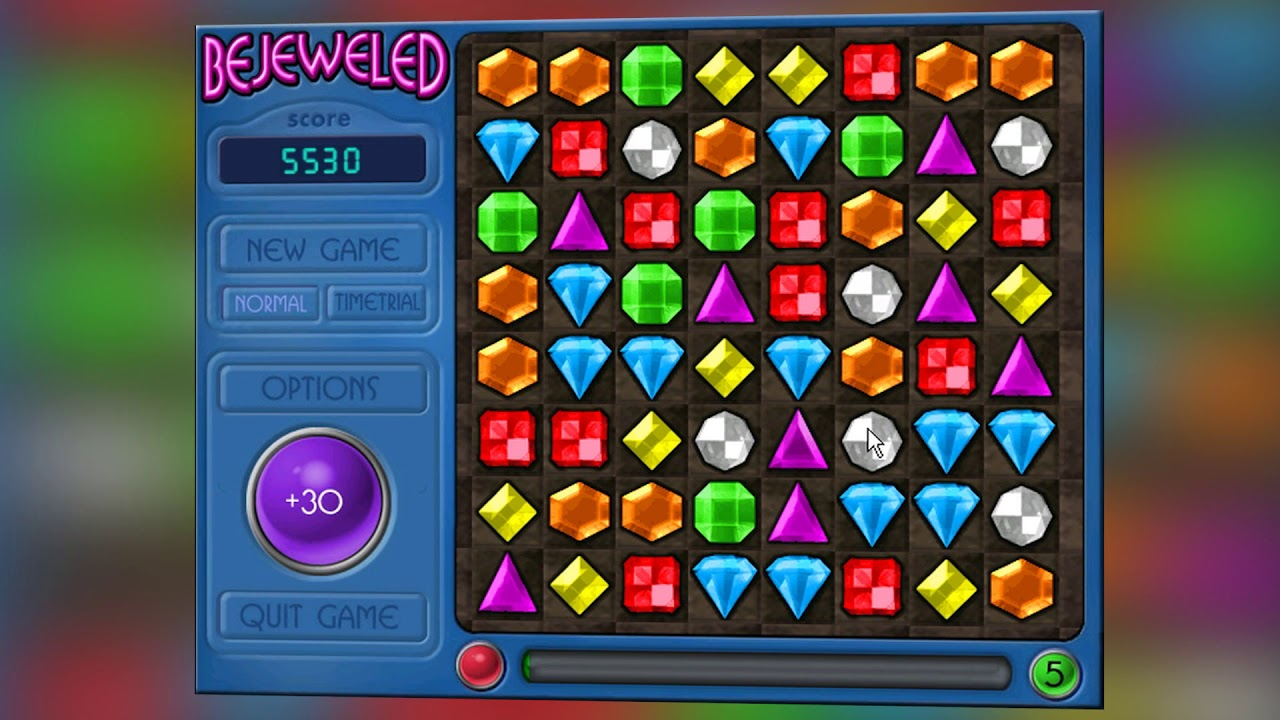
\includegraphics[width=0.9\textwidth]{bejewield}
        \end{frame}

        \begin{frame}
            \frametitle{Match-three concepts}
            \begin{itemize}
                \item Board Representation
                \item Game Logic 
                \item User Interaction
                \item Animation and Graphics
            \end{itemize}
            \end{frame}
        
        \begin{frame}
            \frametitle{Why match-three games}
            \begin{itemize}
                \item Relatively easy to program
                \item Popular 
                \item Work on everything
                \item Graphics dependable
            \end{itemize}
            \end{frame}

    \begin{frame}
        \frametitle{Multiplatform}
        \begin{itemize}
            \item Linux
            \item Windows
            \item Android/iOS
            \item Mac
        \end{itemize}
        \end{frame}

    \section{How}
    \begin{frame}
    \frametitle{Project scope}
    \begin{itemize}
        \item Custom graphics (tiles/backgrounds)
        \item Custom shaders
        \item Defining game rules
        \item Building multiplatform
    \end{itemize}
    \end{frame}
    \begin{frame}
    \frametitle{Technology}
    \begin{itemize}
        \item C++
        \item OpenGL ES (API)
        \item GLFW (windows/input)
        \item GLM (math)
    \end{itemize}
    \end{frame}

    \begin{frame}
        \frametitle{Ease of match 3}
        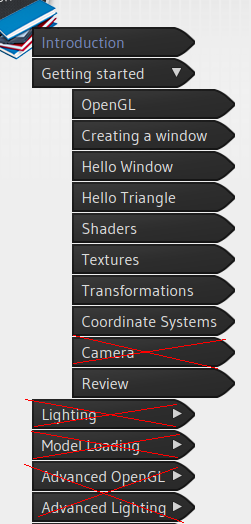
\includegraphics[height=0.6\textwidth]{easy}
        Smaller scope
    \end{frame}

    \begin{frame}
        \frametitle{Engine design overhaul}
        \begin{itemize}
            \item Window/Input management
            \item Graphics/Rendering
            \item Gems attributes
            \item Game Logic 
        \end{itemize}
    \end{frame}

    \begin{frame}
        \frametitle{Window/Input}
        GLFW:
        \begin{itemize}
            \item Create window
            \item Handle input 
            \item Rendering context 
        \end{itemize}
    \end{frame}

    \begin{frame}
        \frametitle{User inputs}
        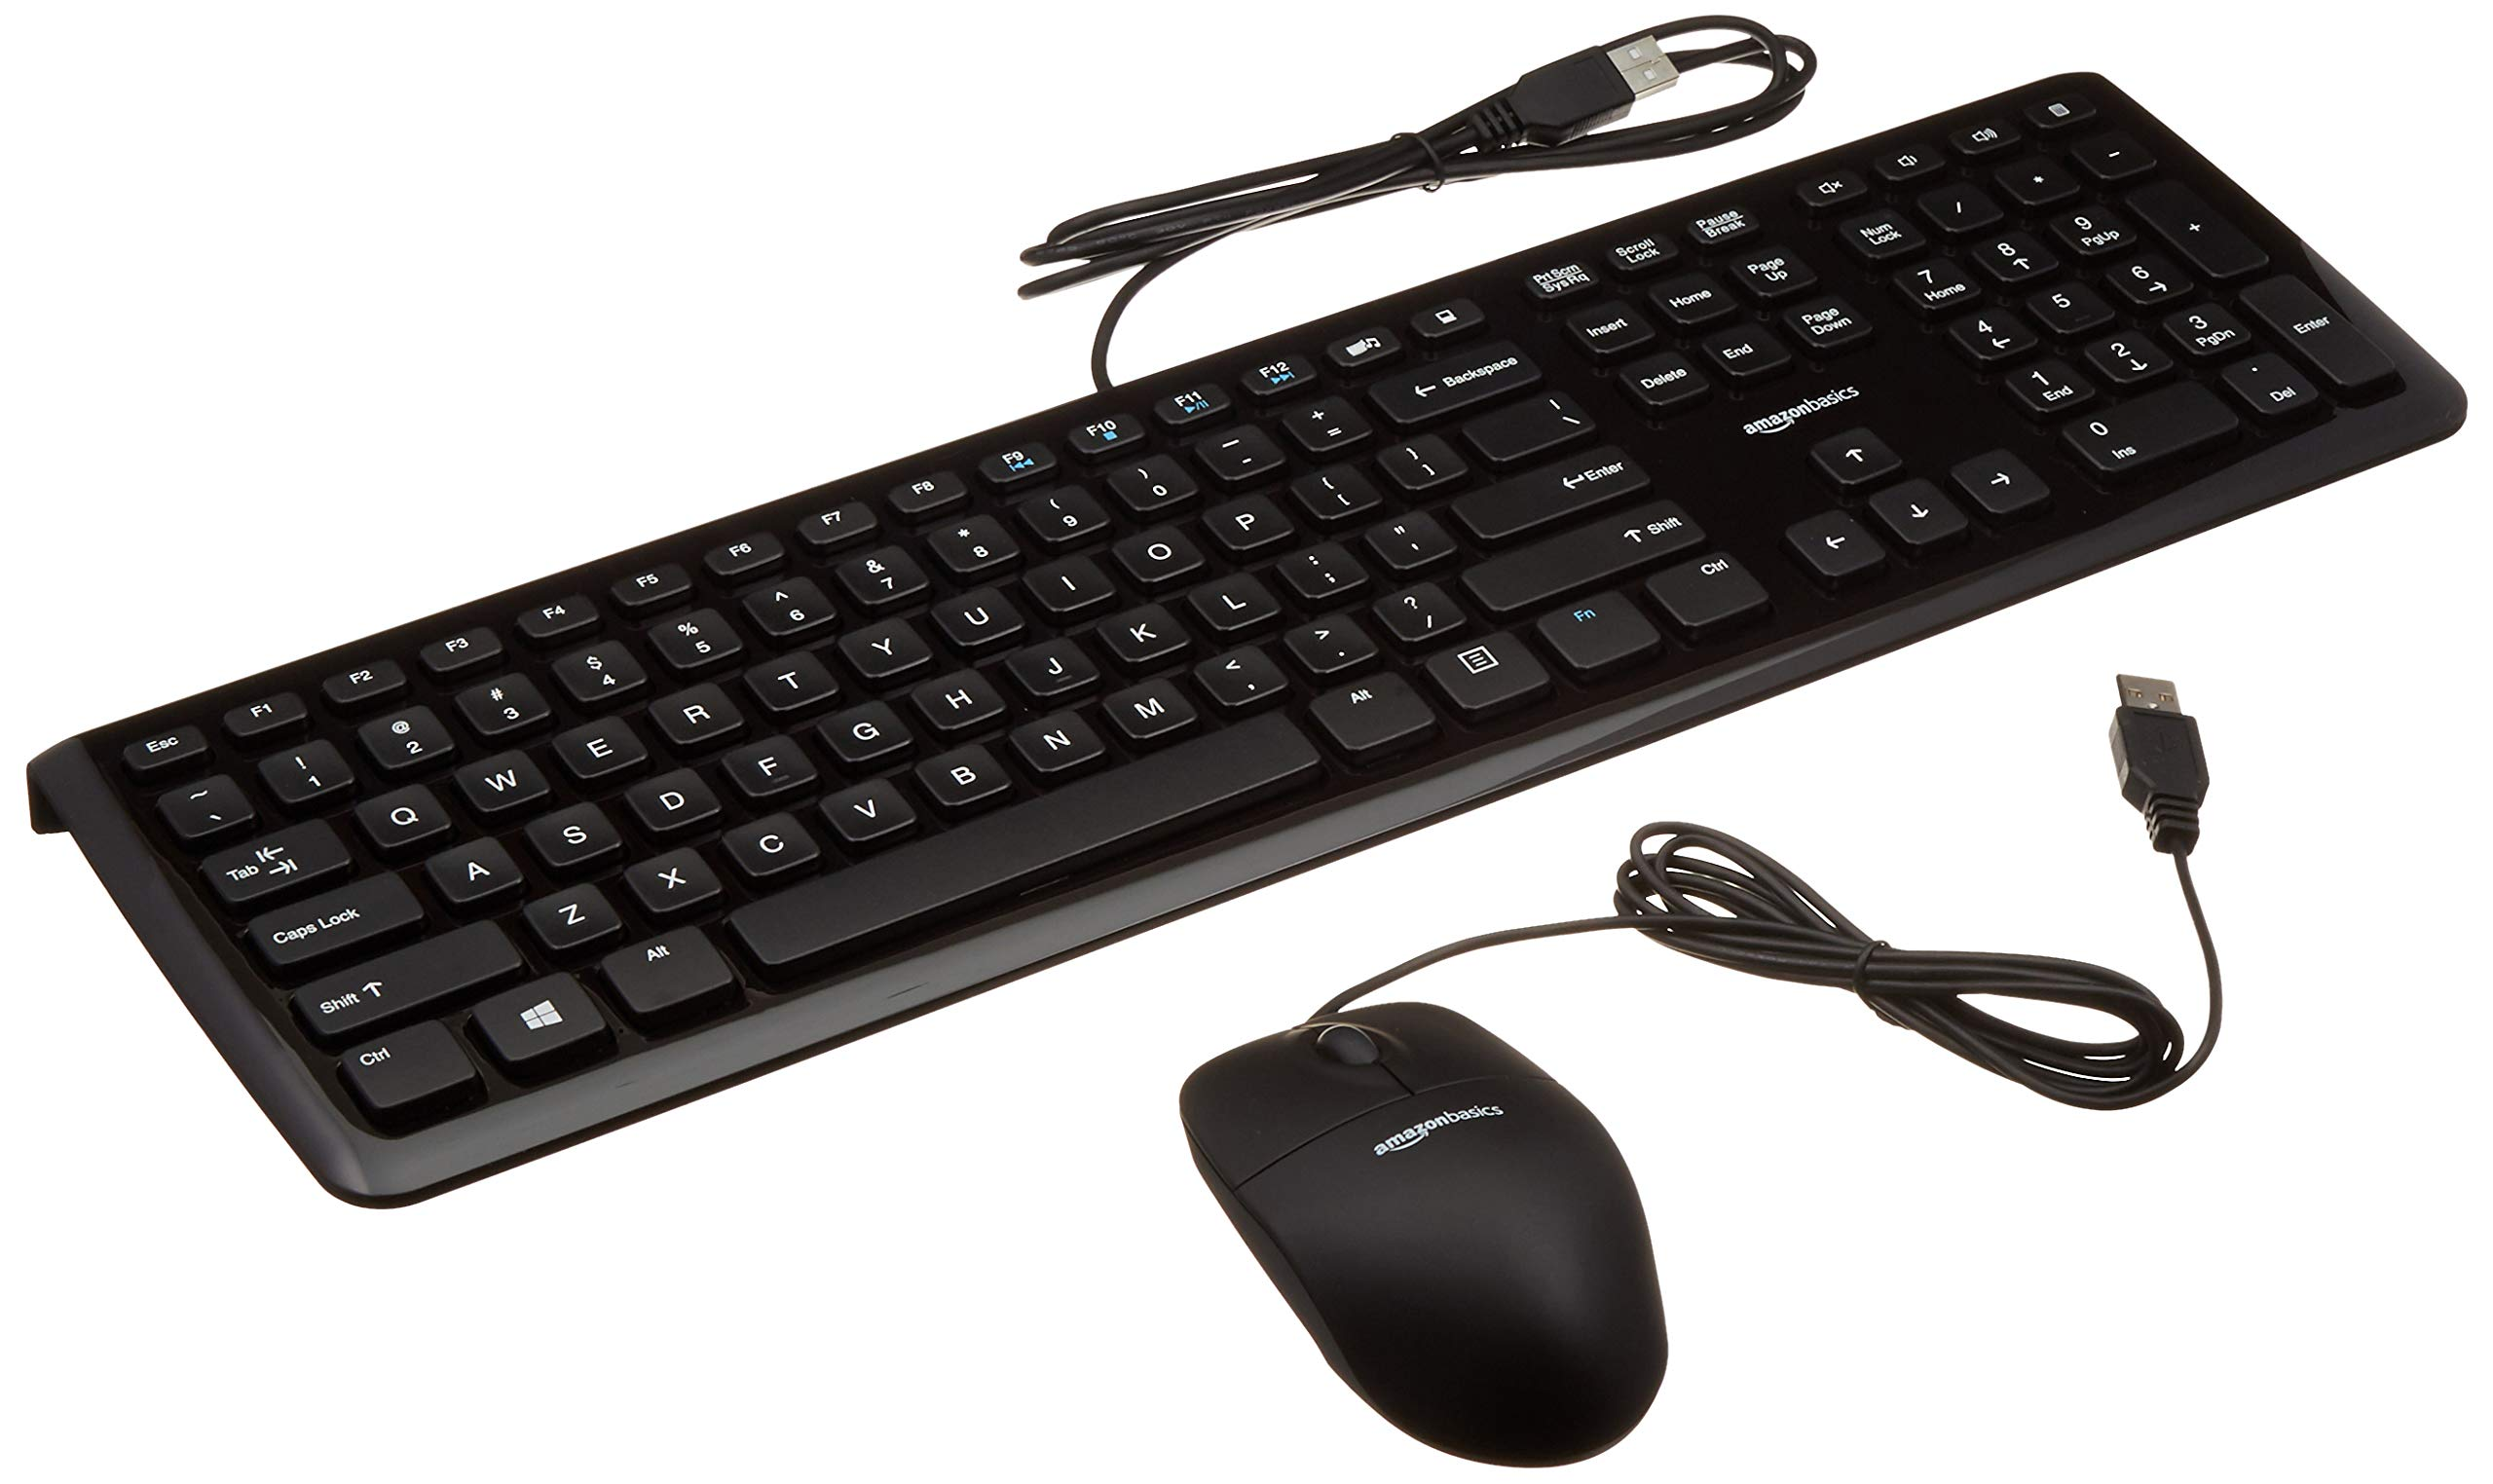
\includegraphics[width=0.4\textwidth]{keyboard.jpg}
        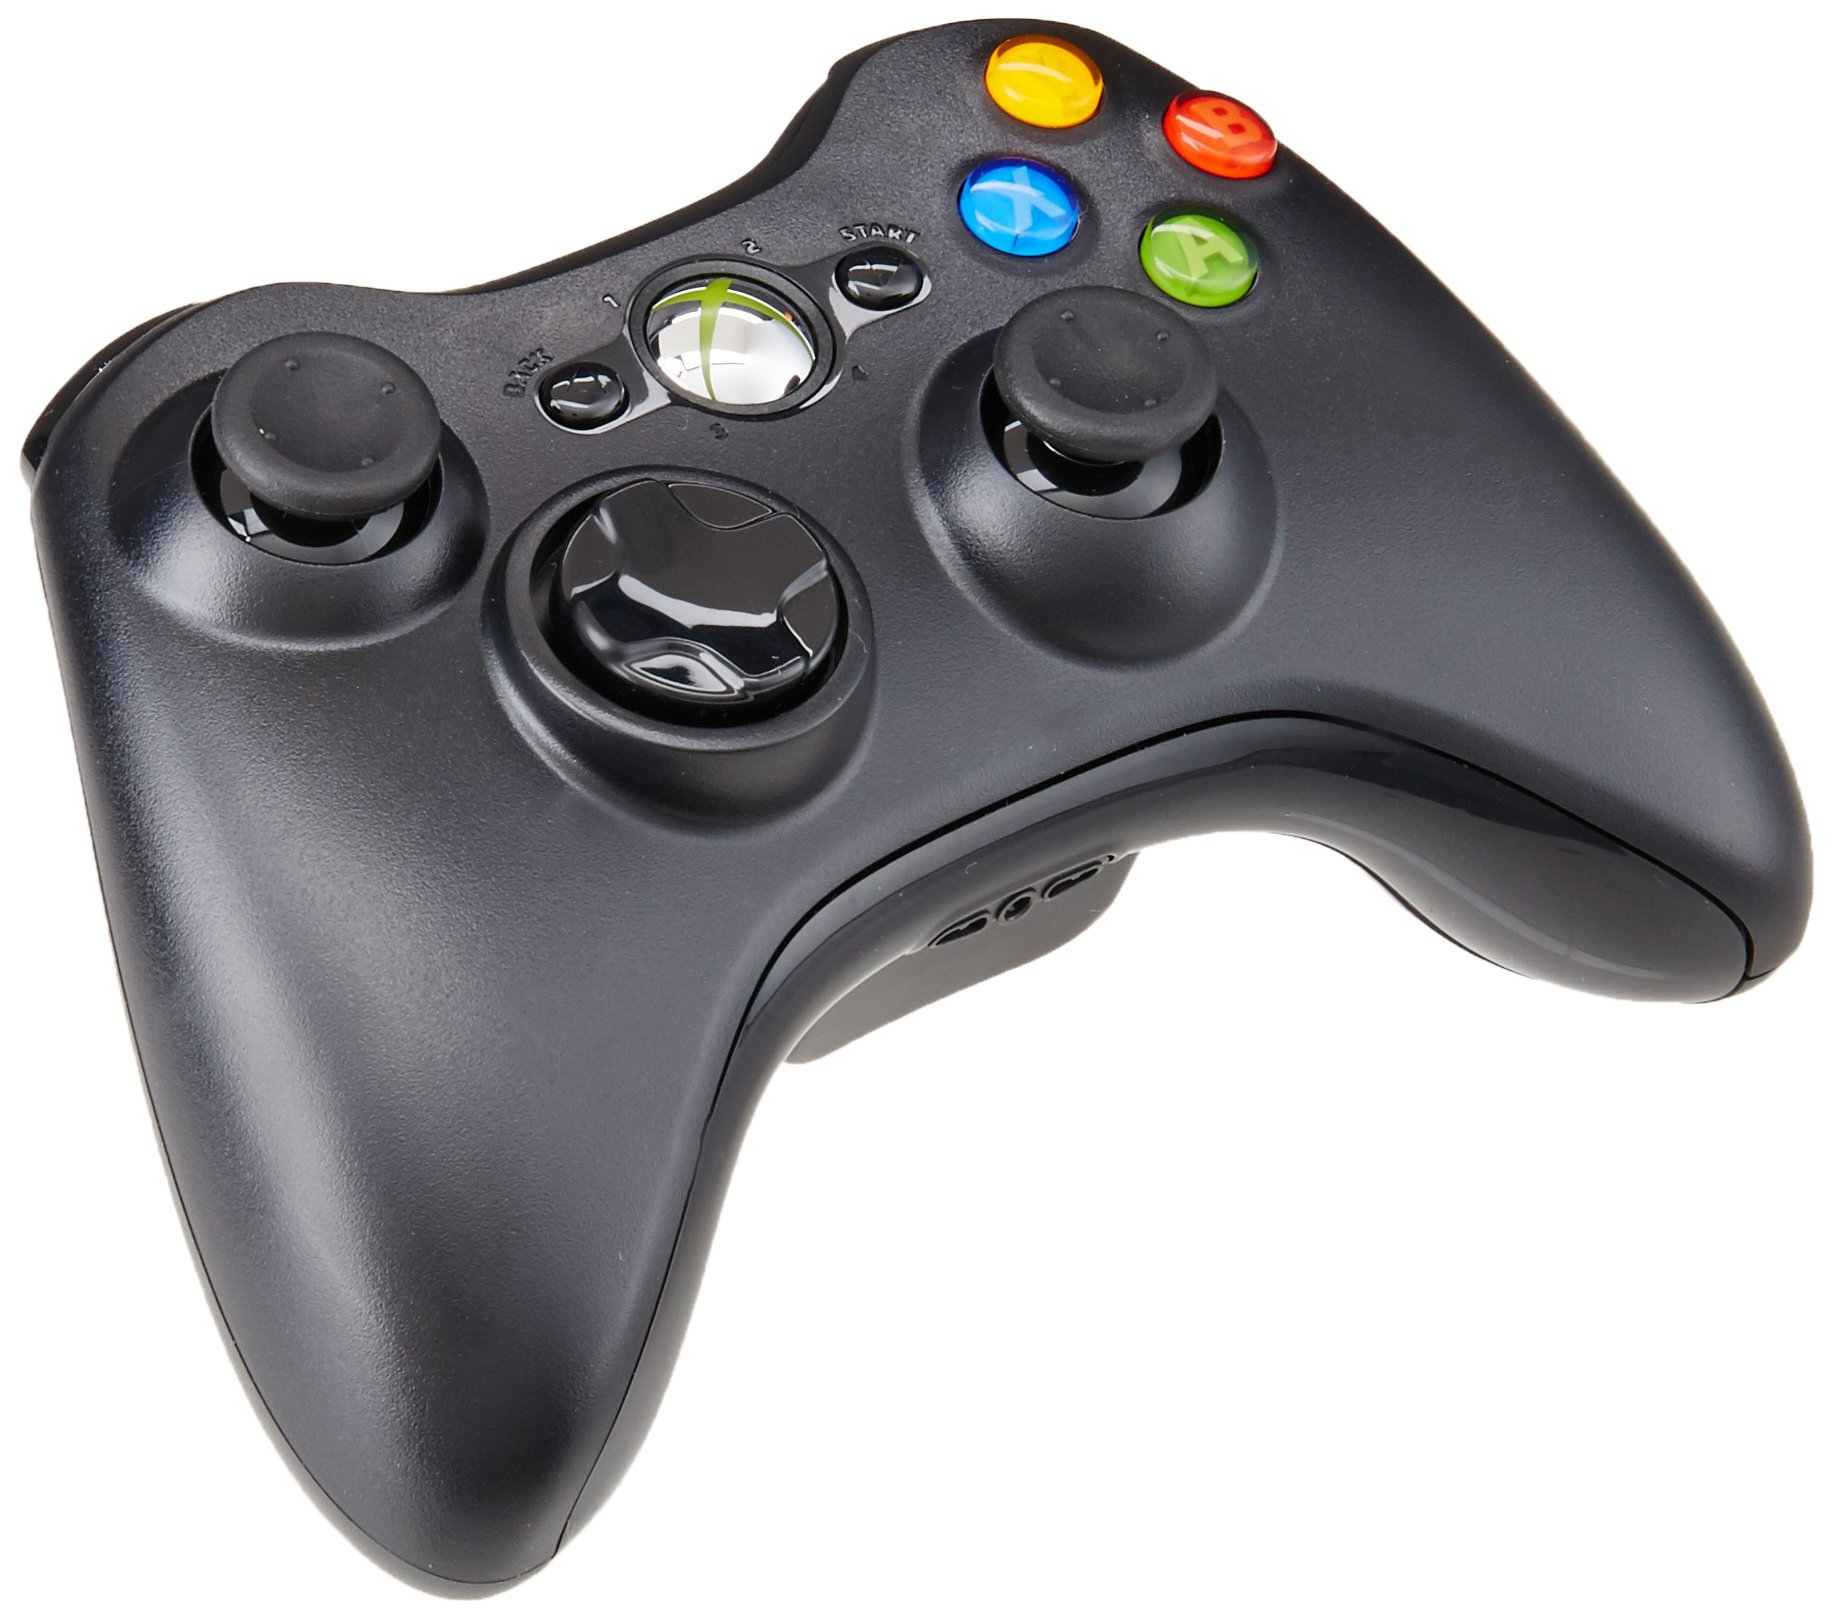
\includegraphics[width=0.4\textwidth]{xbox360.jpg}
        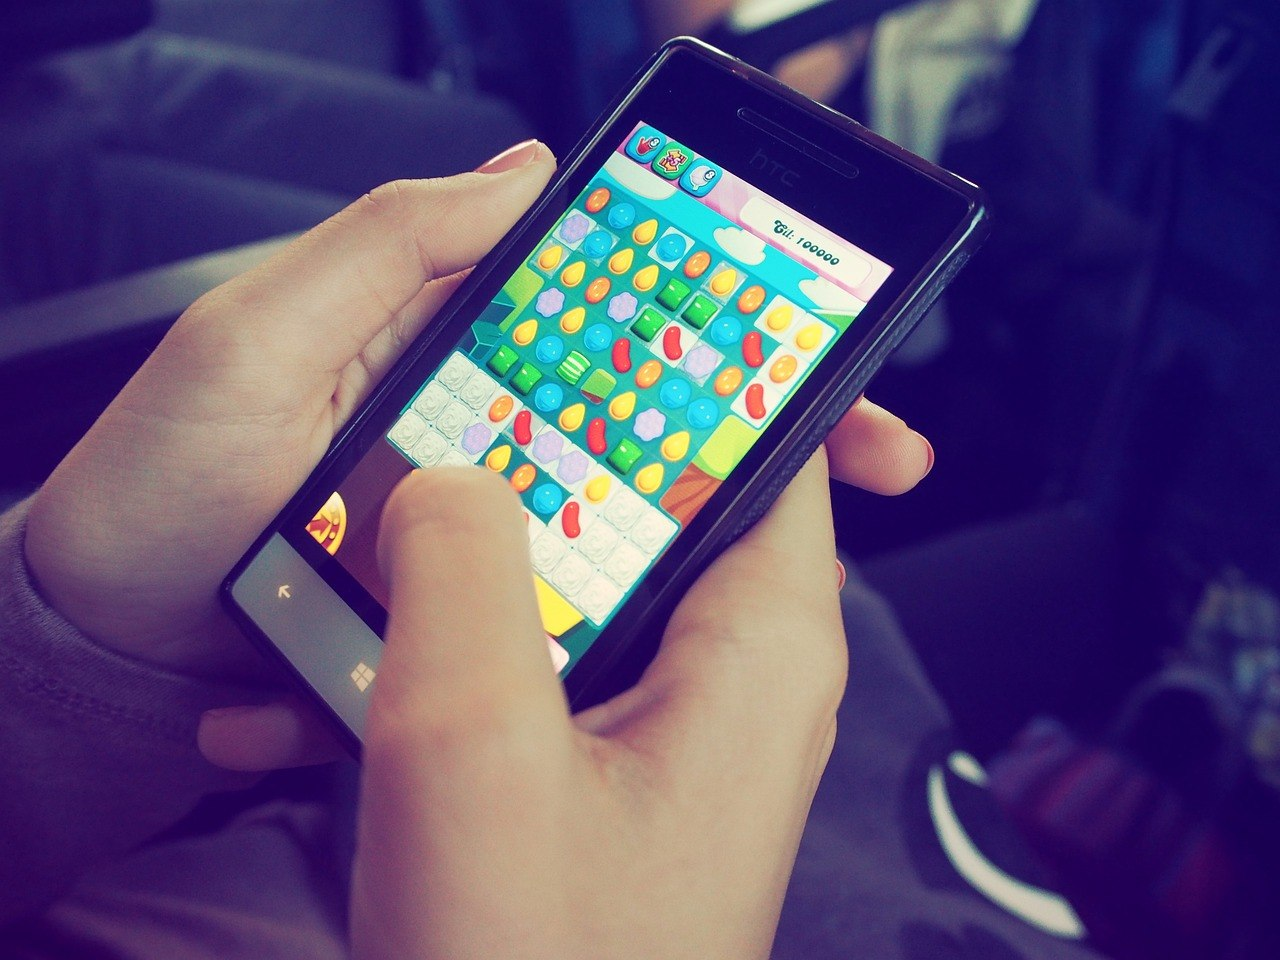
\includegraphics[width=0.4\textwidth]{finger.jpg}
    \end{frame}

    \begin{frame}
        \frametitle{Graphics/Rendering}
        \begin{itemize}
            \item Shaders
            \item Vertex Buffer Objects
            \item Vertex Array Objects
        \end{itemize}
    \end{frame}

    \begin{frame}
        \frametitle{Gems attributes}
        \begin{itemize}
            \item Type
            \item Status 
            \item Position
            \item Value
        \end{itemize}
    \end{frame}

    \begin{frame}
        \frametitle{Game Logic}
        \begin{itemize}
            \item Check for matches
            \item Remove matched
            \item Fill board
        \end{itemize}
    \end{frame}

    \begin{frame}
        \frametitle{Animation}
        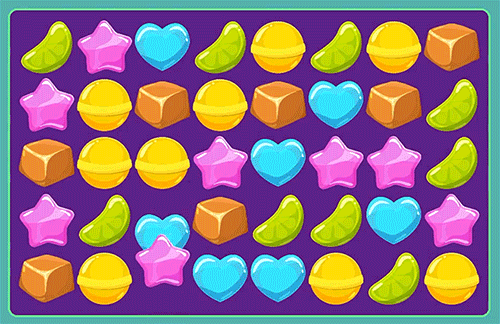
\includegraphics[width=0.9\textwidth]{swap.png}
    \end{frame}



    \section{Summary}
\begin{frame}
    Thesis is about creating a game engine specialized in match-three multiplatform games using OpenGL
    \frametitle{Summary}
    \end{frame}

\section{References}
\begin{frame}
    \begin{itemize}
        \item \href{https://docs.gl/}{https://docs.gl/}
    \item \href{https://learnopengl.com/}{https://learnopengl.com/}
    \item \href{https://www.youtube.com/c/gameengineseries}{The Cherno}
    \item Game Engine Architecture, Jason Gregory
    \end{itemize}
    \frametitle{References/sources}
    \end{frame}

\end{document}